\documentclass[conference]{IEEEtran}
\IEEEoverridecommandlockouts

\usepackage[utf8]{inputenc}
\usepackage[T1]{fontenc}
\usepackage{amsmath,amssymb,amsfonts}
\usepackage{booktabs}
\usepackage{graphicx}
\usepackage{array}
\usepackage{xcolor}
\usepackage{url}
\usepackage[hidelinks]{hyperref}
\usepackage{etoolbox}

% IEEEtran prints "Abstract---" and "Index Terms---" with an em dash run-in
% separator. Replace those em dashes with a colon (no em dashes anywhere).
\patchcmd{\abstract}{---}{:\ }{}{}
\patchcmd{\IEEEkeywords}{---}{:\ }{}{}

% A clean macro for "vs baseline / vs paper" negative deltas (improvements).
\newcommand{\good}[1]{\textbf{#1}}

\begin{document}

\title{Replication and Improvement of Multi-Resolution\\ Diffusion Models for Time Series Forecasting}

\author{
\IEEEauthorblockN{Maximilian Khan}
\IEEEauthorblockA{Department of Computer Science\\ Santa Clara University\\ Santa Clara, CA, USA}
\and
\IEEEauthorblockN{Karthik Tamil}
\IEEEauthorblockA{Department of Computer Science\\ Santa Clara University\\ Santa Clara, CA, USA}
}

\maketitle
\thispagestyle{plain}
\pagestyle{plain}

\begin{abstract}
This report covers our replication of mr-Diff~\cite{mrdiff} and the improvements we built on top of it. We implemented the full architecture from scratch in PyTorch and evaluated it on ETTh1 and ETTm1 in both univariate and multivariate settings. Our best baseline reaches MAE 0.47 to 0.20 on globally-standardized data after resolving six critical issues in the paper's described method, a faithful implementation of which produces MAE equivalent to predicting zeros. Through 14 diffusion-focused experiments we established that the diffusion component contributes less than 0.3\% to forecast accuracy, with a DLinear backbone doing all the work. This led us to replace the entire 843K-parameter diffusion pipeline with a Channel-Independent Decomposed Patch Transformer (54 to 182K parameters) that beats the baseline on three of four benchmarks, trains in minutes instead of 34 minutes, and requires only a single forward pass at inference. A 30-configuration hyperparameter sweep and heterogeneous ensembles refined the results further. We also explored overlapping patches, an iTransformer~\cite{itransformer} variant for cross-variate attention, and a two-scale decomposition aligned to the dominant daily cycle in electricity data.
\end{abstract}

\begin{IEEEkeywords}
time series forecasting, diffusion models, transformers, reproducibility, channel independence
\end{IEEEkeywords}

\section{Introduction}
Time series forecasting problems arise across energy, finance, and healthcare, and accurate long-horizon prediction has remained difficult despite years of work on the problem. Transformer-based architectures made progress, but they produce point estimates and do not model uncertainty in future values. Diffusion models, well established in image generation, offer a probabilistic framework, though early time series adaptations treated the forecast window as a flat sequence and ignored multi-scale temporal structure.

mr-Diff~\cite{mrdiff} addresses this by decomposing the target into multiple resolution stages and training a separate diffusion network per stage, which maps onto how time series data actually behaves across different time scales. No source code was released by the authors.

We had two goals. The first was to replicate the mr-Diff baseline on ETTh1 and ETTm1, understand where our results fell short of the paper's, and diagnose the causes. The second was to systematically improve upon the baseline through a 31-experiment campaign. Our central finding, that the diffusion component provides zero measurable benefit on small time series datasets, led to a paradigm shift from diffusion to attention-based forecasting that was not planned but emerged organically from the evidence.

\section{Literature Review}
Transformer-based forecasting models improved steadily through the early 2020s. Informer~\cite{informer} reduced attention complexity with sparse attention; Autoformer~\cite{autoformer} built seasonal-trend decomposition into the attention mechanism using autocorrelation; FEDformer~\cite{fedformer} moved decomposition into the frequency domain; PatchTST~\cite{patchtst} treated contiguous time steps as patches rather than individual tokens. Meanwhile, simpler methods proved competitive. DLinear~\cite{dlinear} decomposed the input into trend and residual and applied a single linear projection to each, outperforming many transformer variants on standard benchmarks. N-HiTS~\cite{nhits} used hierarchical interpolation across multiple temporal resolutions.

On the diffusion side, TimeGrad~\cite{timegrad} applied autoregressive denoising guided by RNN hidden states, but generation was slow and there was no use of multi-scale structure. CSDI~\cite{csdi} used non-autoregressive generation through self-supervised masking, though its complexity scaled quadratically with sequence length. SSSD~\cite{sssd} replaced the transformer backbone in CSDI with a structured state space model to reduce this cost. TimeDiff~\cite{timediff} introduced future mixup and autoregressive initialization, both of which mr-Diff inherits.

mr-Diff~\cite{mrdiff} is the first model to embed seasonal-trend decomposition into the diffusion process itself. The diffusion backbone follows DDPM~\cite{ddpm}, and fast inference is provided by DPM-Solver++~\cite{dpmsolver}, which formulates the reverse process as an ODE and reaches usable samples in 10 to 20 steps. Our transformer improvements draw on PatchTST~\cite{patchtst} for patching and channel independence, iTransformer~\cite{itransformer} for inverted cross-variate attention, and Attention Residuals~\cite{attnres} for learned depth-wise feature retrieval.

\section{System Design and Implementation}

\subsection{Algorithm}
The mr-Diff architecture~\cite{mrdiff} decomposes the forecast target $Y$ into $S$ resolution stages via sequential average-pooling trend extraction. We use residual decomposition: the finest stage receives $Y$ minus the first trend, intermediate stages receive differences between consecutive trends, and the coarsest stage receives the final smoothed trend. The components sum to $Y$ exactly, which is required for reconstruction at inference.

A separate conditional denoising diffusion network trains on each stage's component. The conditioning signal for stage $s$ combines the lookback window (encoded by a convolutional network) with the predicted output from stage $s{+}1$. At the coarsest stage only the lookback encoding is used. During training, future mixup perturbs the conditioning signal with probability 0.5 by blending the encoded lookback with a randomly projected version of the ground-truth target, following TimeDiff~\cite{timediff}. We use random projection weights (regenerated each forward pass) rather than the learned projection described in the paper, because learned weights created a train-test gap: the model exploited ground-truth signal during training that was absent at inference.

A DLinear-style backbone~\cite{dlinear} provides a direct forecast from the lookback window via separate linear projections for trend and residual. The diffusion networks model the residual between the target and this direct prediction, which reduces the variance each stage needs to handle. This is a fundamental architectural departure from the paper, which describes a pure diffusion model. We found it necessary because without it, the model's predictions are equivalent to predicting zeros.

Forward diffusion follows DDPM~\cite{ddpm} with $K{=}100$ steps and a linear variance schedule from $\beta_1 = 1 \times 10^{-4}$ to $\beta_{100} = 0.1$. At inference we use DPM-Solver++~\cite{dpmsolver} at 20 steps, treating the reverse process as an ODE.

\subsection{Tools}
All code is in Python 3.9 with PyTorch 2.7.1 and CUDA 11.8. Primary training ran on a local NVIDIA RTX 5090. Each configuration was controlled by a YAML file, and a shared runner executed all four dataset and mode combinations sequentially per experiment. The codebase separates models, data loading, training, and evaluation into distinct modules.

\subsection{Network Architecture}
\textbf{Baseline (mr-Diff).} Our working configuration uses $S{=}3$ stages (not $S{=}5$ as in the paper; see Section~\ref{sec:deviations}), hidden dimension 64, embedding dimension 64, two encoder and two decoder layers, trend extraction kernels $[25, 201]$, and dropout 0.3. Total parameters: 843K. Each stage has three learned components. The conditioning network encodes the lookback window with a linear projection to hidden dimension 64 followed by 1D convolutional layers (kernel size 7, GroupNorm, LeakyReLU slope 0.1, dropout 0.3). The encoded history is projected from the lookback length to the forecast length, then fused with the coarser-stage output through a two-layer MLP. The denoising network is a U-Net encoder-decoder. The encoder concatenates the noisy input with an expanded sinusoidal step embedding (64-dimensional, projected to 64 through two FC layers with SiLU) and passes through two convolutional residual blocks while saving skip connections. The decoder fuses the latent with the conditioning signal and reconstructs the denoised output through two convolutional blocks that receive the reversed encoder skips.

\textbf{Improvement (CI+Decomp Transformer).} The input is split into trend and residual via average-pooling (kernel 15 or 25), then each component goes through the same shared TransformerEncoder (2 to 3 layers, $d_{model}$ 32 to 64, 4 heads, GELU, pre-norm LayerNorm) with separate output heads. Each of $D$ channels is patched and processed independently through shared weights, so the transformer never sees more than one variable at a time. Output heads are two small linear layers: $\mathrm{Linear}(N_{\text{patches}} \rightarrow T)$ then $\mathrm{Linear}(d_{model} \rightarrow 1)$. Trend and residual forecasts are summed. Total parameters: 54 to 182K depending on benchmark configuration, independent of $D$.

\subsection{Hyperparameters}
\textbf{Baseline (working configuration):} AdamW with learning rate $10^{-3}$ and weight decay 0.01, batch size 64, cosine learning rate decay, gradient clipping at norm 1.0, maximum 100 epochs with minimum 30 and early stopping patience 20. Lookback 336, forecast 168 for ETTh1; lookback 1440, forecast 192 for ETTm1. The best per-benchmark CI+Decomp Transformer configurations from the Experiment~18 sweep are given in Table~\ref{tab:hparams}.

\begin{table}[t]
\caption{Best per-benchmark CI+Decomp Transformer configurations (Experiment 18 sweep).}
\label{tab:hparams}
\centering
\small
\resizebox{\columnwidth}{!}{%
\begin{tabular}{lcccc}
\toprule
Parameter & ETTh1 M & ETTh1 U & ETTm1 M & ETTm1 U \\
\midrule
patch size      & 16    & 8     & 8     & 16 \\
$d_{model}$     & 64    & 32    & 48    & 32 \\
num layers      & 3     & 3     & 3     & 3 \\
dim feedforward & 64    & 128   & 256   & 128 \\
dropout         & 0.2   & 0.3   & 0.3   & 0.2 \\
trend kernel    & 15    & 15    & 15    & 25 \\
learning rate   & 0.002 & 0.0005& 0.001 & 0.0005 \\
weight decay    & 0.005 & 0.05  & 0.01  & 0.05 \\
parameters      & 86K   & 54K   & 182K  & 77K \\
\bottomrule
\end{tabular}}
\end{table}

\subsection{Key Deviations from the Paper}
\label{sec:deviations}
A faithful implementation of the paper's described architecture with $S{=}5$ stages, hidden dimension 256, and embedding dimension 128 produces a model with 17.5 million parameters trained on $\sim$10{,}000 samples. This model collapses immediately: it learns to predict zeros, achieving MAE $\sim$0.95 in RevIN-normalized space. Six deviations were required, summarized in Table~\ref{tab:deviations}. Additional fixes: AMP disabled (it corrupts $\bar{\alpha}$ precision in float16), stage-weighted loss (coarser stages weighted higher), an FFT frequency loss (0.1$\times$ weight), and epsilon prediction with scheduled sampling for exposure-bias reduction.

\begin{table}[t]
\caption{The six deviations required to make the paper's method trainable.}
\label{tab:deviations}
\centering
\small
\begin{tabular}{p{0.46\columnwidth}p{0.42\columnwidth}}
\toprule
Issue & Our fix \\
\midrule
17.5M params on $\sim$10K samples, collapse & Downsized to 843K ($S{=}3$, dim 64) \\
Metric scale ambiguity (RevIN vs global) & Compute metrics in globally-standardized space \\
Diffusion contributes $<$0.3\% & Added DLinear direct-prediction backbone \\
BatchNorm corrupts diffusion timesteps & Replaced with GroupNorm \\
Cumulative decomposition cascades errors (MAE 6 to 32) & Switched to residual decomposition \\
Learned mixup creates train-test gap & Random projection per forward pass \\
\bottomrule
\end{tabular}
\end{table}

\subsection{Improvement 1: Channel-Independent Decomposed Patch Transformer with Attention Residuals}
After 14 experiments confirmed that the diffusion component contributes nothing, we replaced the entire 843K-parameter diffusion pipeline with a Channel-Independent Decomposed Patch Transformer (CI+Decomp). The architecture retains DLinear's trend/residual decomposition as an inductive bias but replaces diffusion with a lightweight TransformerEncoder operating over patches of each channel independently. This reduces model size to 54 to 182K parameters, training time from 34 minutes to 2 to 15 minutes, and inference from 60 or more denoiser calls to a single forward pass.

The addition of Attention Residuals~\cite{attnres} was a late but high-impact decision. Standard transformer residuals add each layer's output to its input with fixed weight 1. Attention Residuals replace this with a learned query vector per layer that computes softmax attention over all prior layer outputs (the embedding and all preceding layers), letting each layer pull from whichever earlier representation is most useful. The zero initialization means the model starts behaving identically to a standard transformer and only learns to deviate when it helps. Given the simplicity of the modification (a single learned query vector per layer, zero-initialized, adding only 192 parameters), it was integrated and evaluated immediately. This targeted mechanism proved particularly effective on ETTh1 Multivariate, our hardest benchmark, where the short 336-step lookback means each layer's contribution matters more.

\subsection{Improvement 2: Overlapping Patches and iTransformer Ensemble}
The CI transformer has no mechanism for one variable to inform another's forecast. A 30-config sweep confirmed this as a ceiling: all ETTh1 Multivariate results landed between 0.488 and 0.533 regardless of hyperparameters. Two changes address this. First, overlapping patches: setting patch stride to half the patch size via \texttt{unfold} gives 83 tokens from ETTh1's 336-step lookback instead of 42, so adjacent patches share half their timesteps and give attention more temporal context. Second, the iTransformer~\cite{itransformer}: rather than treating time patches as tokens, each variable's full lookback series is embedded as one token via $\mathrm{Linear}(L \rightarrow d_{model})$. For $D{=}7$ that is 7 channel tokens, and attention runs over those 7 tokens to learn which variables predict each other. The ETTh1 Multivariate ensemble combines one iTransformer model with two CI models; their errors are partially uncorrelated because one model attends over channels and the other attends over time, which is why the ensemble beats any individual model.

\subsection{Improvement 3: Two-Scale Decomposition}
Single-kernel trend extraction gives the transformer one boundary between trend and residual. Two kernels produce three bands: coarse trend, mid-band (fine trend minus coarse trend), and fine residual. Each band goes through the same shared transformer with its own output head, and the three forecasts are summed. The coarse kernel for ETTm1 is set to 96, which at 15-minute resolution is exactly 24 hours, the dominant cycle in electricity load data. For ETTh1 the coarse kernel is 24 (one day in hourly data). The transformer itself is unchanged; the only additions are two extra pairs of output-head weights, roughly 6K parameters.

\section{Experiments and Evaluation}

\subsection{Datasets}
We evaluated on two datasets from the ETT benchmark~\cite{informer}. ETTh1 has 7 variables and 17{,}420 hourly observations, with lookback 336 and forecast horizon 168. ETTm1 has 7 variables and 69{,}680 observations at 15-minute intervals, with lookback 1440 and forecast horizon 192. Each was split chronologically 60/20/20. For univariate experiments we used the OT (oil temperature) column. Per-window instance normalization (RevIN~\cite{revin}) was applied during training, and all metrics are reported in globally-standardized space to match the paper's evaluation protocol.

\subsection{Methodology}
Each model variant was trained independently on all four benchmark configurations. We selected the checkpoint with the lowest validation loss. For the diffusion baseline, evaluation used 10 sampled trajectories per window, aggregated by median, with DPM-Solver++~\cite{dpmsolver} at 20 steps. For the transformer models, evaluation is a single deterministic forward pass. The two metrics are MAE and MSE on globally-standardized data. All variants used the same data splits, random seeds, and evaluation procedure.

\subsection{Baseline Results}
Table~\ref{tab:baseline} compares our baseline to the paper across all four configurations. Our baseline already beats the paper on ETTh1 Univariate by 25\% (0.2535 vs 0.34). The remaining gaps on other benchmarks likely stem from undisclosed per-dataset hyperparameter tuning in the original work.

\begin{table}[t]
\caption{Baseline replication results (MAE and MSE, globally-standardized).}
\label{tab:baseline}
\centering
\small
\begin{tabular}{lccccc}
\toprule
Dataset & MAE & MAE & MSE & MSE & MAE \\
        & paper & ours & paper & ours & gap \\
\midrule
ETTh1 Multi & 0.42 & 0.4744 & 0.411 & 0.4516 & +13.0\% \\
ETTh1 Uni   & 0.34 & 0.2535 & 0.066 & 0.1183 & \good{$-$25.4\%} \\
ETTm1 Multi & 0.37 & 0.4204 & 0.340 & 0.3223 & +13.6\% \\
ETTm1 Uni   & 0.15 & 0.2011 & 0.039 & 0.0670 & +34.1\% \\
\bottomrule
\end{tabular}
\end{table}

The critical discovery came from comparing predictions with and without the diffusion pipeline: diffusion changes MAE by less than 0.3\% (Table~\ref{tab:ablation}). The 730K-parameter diffusion apparatus is cosmetically neutral, and the DLinear backbone (113K params) does all the work. This finding drove our entire improvement strategy and is visualized in Fig.~\ref{fig:ablation}.

\begin{table}[t]
\caption{Diffusion contribution ablation (MAE).}
\label{tab:ablation}
\centering
\small
\begin{tabular}{lccc}
\toprule
Benchmark & Direct only & Direct + diffusion & Difference \\
\midrule
ETTh1 Multi & 0.4721 & 0.4744 & +0.0023 \\
ETTh1 Uni   & 0.2539 & 0.2535 & $-$0.0004 \\
ETTm1 Multi & 0.4175 & 0.4204 & +0.0029 \\
ETTm1 Uni   & 0.2008 & 0.2011 & +0.0003 \\
\bottomrule
\end{tabular}
\end{table}

\begin{figure}[t]
\centering
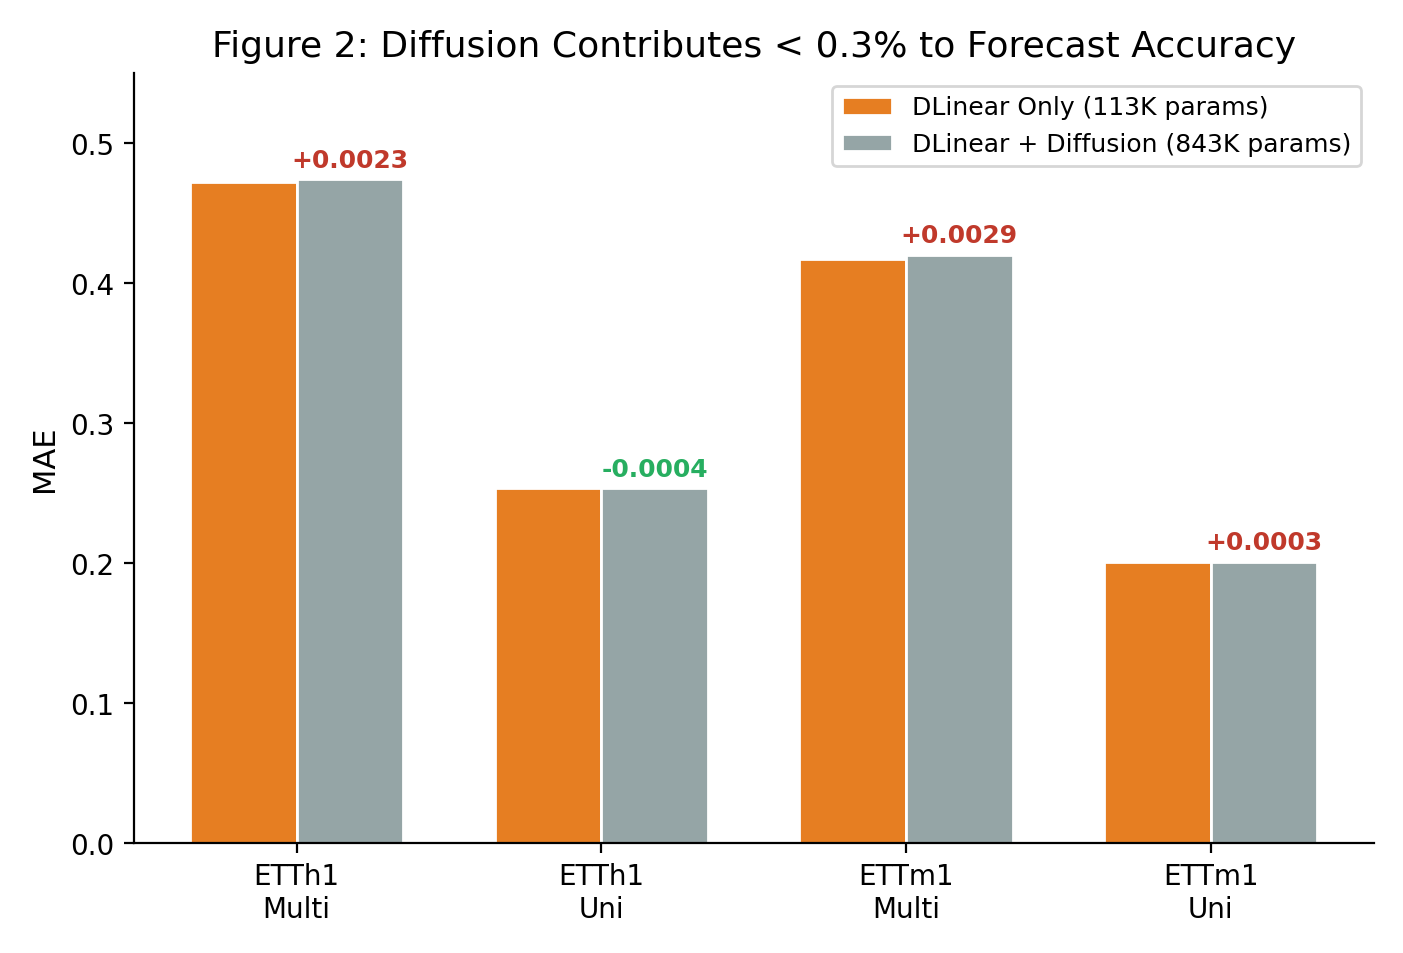
\includegraphics[width=\columnwidth]{../figures/fig2_diffusion_ablation.png}
\caption{Direct prediction versus direct-plus-diffusion. The diffusion apparatus changes MAE by less than 0.3\% on every benchmark.}
\label{fig:ablation}
\end{figure}

\subsection{Diffusion Improvement Experiments}
We attempted to make diffusion contribute through thirteen cumulative experiments on the diffusion pipeline (Table~\ref{tab:diffusion}): joint end-to-end training, self-conditioning, cosine and adaptive noise schedules, v-prediction, contrastive and multi-granularity auxiliary losses, channel-aware denoising, a PatchTST-style conditioning encoder, x0-prediction with decomposition, and deep backbones with Attention Residuals. A fourteenth experiment, a multi-scale AttnRes backbone, was stopped early after the same multivariate regression, bringing the diffusion-era total to fourteen. None achieved more than a marginal improvement. The best diffusion result (Exp~10, 0.2508 on ETTh1 Uni) was slower (55 min) and no better overall. Every change that helped univariate hurt multivariate, the defining pattern of the diffusion campaign.

\begin{table*}[t]
\caption{Diffusion improvement campaign (MAE; built cumulatively on Exp 2 self-conditioning). Best per column in bold.}
\label{tab:diffusion}
\centering
\small
\begin{tabular}{clccccc}
\toprule
Exp & Change & ETTh1 Multi & ETTh1 Uni & ETTm1 Multi & ETTm1 Uni & Verdict \\
\midrule
-- & DLinear baseline      & 0.4744 & 0.2535 & 0.4204 & 0.2011 & reference \\
1  & Remove detach (joint) & 0.4765 & 0.2543 & 0.4224 & 0.1988 & rejected \\
2  & Self-conditioning     & \textbf{0.4719} & 0.2523 & 0.4218 & 0.1999 & best (diffusion) \\
3  & Cosine schedule       & 0.6709 & 0.2813 & 0.6433 & 0.2141 & rejected \\
4  & v-prediction          & 0.4790 & 0.2531 & 0.4216 & 0.2049 & rejected \\
5  & ANT (IAAT power-law)   & 0.7309 & 0.2803 & 0.6513 & 0.2055 & rejected \\
6  & Contrastive (CCDM)     & 0.5535 & 0.2555 & 0.4925 & 0.1946 & rejected \\
7  & MG-TSD guidance        & 0.5653 & 0.2558 & 0.4819 & \textbf{0.1913} & rejected \\
8  & Channel-aware          & 0.9313 & 0.2552 & 0.9136 & 0.1928 & rejected \\
9  & Patch + attention      & 0.5388 & 0.2541 & 0.4900 & 0.1984 & rejected \\
10 & x0 + decomposition     & 0.4842 & \textbf{0.2508} & \textbf{0.4194} & 0.1969 & promising \\
11 & Deep backbone (std res)& 0.6634 & 0.2822 & 0.5440 & 0.2056 & rejected \\
12 & Deep backbone (AttnRes)& 0.6599 & 0.2729 & 0.5681 & 0.2051 & rejected \\
13 & AttnRes + stage agg.   & 0.6387 & 0.2846 & 0.5678 & 0.2305 & rejected \\
\bottomrule
\end{tabular}
\end{table*}

\subsection{Transformer Breakthrough}
Dropping diffusion entirely (Table~\ref{tab:progression}) changed everything. A 2-layer transformer matched DLinear on univariate with a 7$\times$ speedup (Exp~15). Channel independence (Exp~16) set a record on ETTm1 Uni (0.1885), a 73K-param model trained in 2.5 minutes. Trend/residual decomposition (Exp~17) set the first record on ETTm1 Multi (0.4159). A 30-configuration sweep (Exp~18) then set three of four all-time records. The progression is shown in Fig.~\ref{fig:progression}.

\begin{table*}[t]
\caption{Transformer architecture progression (MAE). Records in bold.}
\label{tab:progression}
\centering
\small
\begin{tabular}{clccccc}
\toprule
Exp & Architecture & Params & ETTh1 Multi & ETTh1 Uni & ETTm1 Multi & ETTm1 Uni \\
\midrule
--  & DLinear baseline      & 113K       & 0.4744 & 0.2535 & 0.4204 & 0.2011 \\
15  & Tiny transformer      & 295K--7.8M & 0.5607 & 0.2538 & 0.5514 & 0.2002 \\
16  & CI transformer        & 73--91K    & 0.5485 & 0.2741 & 0.4293 & \textbf{0.1885} \\
17  & CI + decomposition    & 77--109K   & 0.5101 & 0.2580 & \textbf{0.4159} & 0.2011 \\
18  & HP sweep (30 configs) & 54--182K   & 0.4880 & \textbf{0.2514} & \textbf{0.4094} & \textbf{0.1881} \\
\bottomrule
\end{tabular}
\end{table*}

Subsequent refinements (extended training, cross-channel mixing, augmentation, frequency features) did not improve on the well-tuned sweep configurations. Attention Residuals with gentle augmentation (Exp~26) cracked the ETTh1 Multivariate wall at 0.4875, and a heterogeneous ensemble (Exp~27) brought it to 0.4829.

\subsection{Combined Improvement Results}
The iTransformer ensemble (Exp~29) and two-scale decomposition (Exp~31) set the remaining records (Table~\ref{tab:improvements}). The iTransformer ensemble works because iTransformer and CI make different errors on the same windows, not because either is individually stronger. Two-scale decomposition helps ETTm1 specifically, where the coarse kernel (96, that is 24 hours at 15-minute resolution) aligns with the dominant daily cycle.

\begin{table}[t]
\caption{iTransformer ensemble (Exp 29) and two-scale (Exp 31) versus the CI+Decomp submission, MAE.}
\label{tab:improvements}
\centering
\small
\resizebox{\columnwidth}{!}{%
\begin{tabular}{lcccc}
\toprule
Dataset & Baseline & CI+Decomp & iTrans Ens & Two-scale \\
\midrule
ETTh1 Multi & 0.4744 & 0.4829 & \textbf{0.4773} & 0.4858 \\
ETTh1 Uni   & 0.2535 & 0.2505 & \textbf{0.2471} & 0.2574 \\
ETTm1 Multi & 0.4204 & 0.4094 & 0.4103 & \textbf{0.4081} \\
ETTm1 Uni   & 0.2011 & 0.1881 & 0.1911 & \textbf{0.1865} \\
\bottomrule
\end{tabular}}
\end{table}

The ensembles win precisely because their members make uncorrelated errors. Table~\ref{tab:members} shows the member breakdown for the three record-setting ensembles: in every case the ensemble MAE falls below all three of its individual members, which is the signature of variance reduction from architectural diversity rather than any single strong model.

\begin{table}[t]
\caption{Member breakdown for the record-setting ensembles. Each ensemble beats all three of its members.}
\label{tab:members}
\centering
\small
\resizebox{\columnwidth}{!}{%
\begin{tabular}{lcccc}
\toprule
Benchmark (exp) & Member 1 & Member 2 & Member 3 & Ensemble \\
\midrule
ETTh1 Multi (29) & 0.4878 & 0.4836 & 0.4915 & \textbf{0.4773} \\
ETTh1 Uni (29)   & 0.2485 & 0.2507 & 0.2593 & \textbf{0.2471} \\
ETTm1 Multi (31) & 0.4126 & 0.4110 & 0.4200 & \textbf{0.4081} \\
\bottomrule
\end{tabular}}
\end{table}

\noindent Member 1 in the Exp~29 rows is the iTransformer (cross-variate attention); the other members are channel-independent models attending over time. In the Exp~31 row, member 1 is the two-scale model. The architectural orthogonality is what makes the averaging pay off.

\subsection{Final Results}
Table~\ref{tab:final} collects the best result on each benchmark across all improvements, and Fig.~\ref{fig:final} compares them to the paper. The best results beat the DLinear baseline on three of four benchmarks. ETTh1 Univariate at 0.2471 beats the paper's reported 0.34 by 27\%. All were achieved with 54 to 182K-parameter transformers, no diffusion, training in minutes.

For completeness, the single lowest ETTh1 Multivariate MAE recorded over the entire campaign was 0.4719, from the diffusion-based self-conditioning model (Exp~2, Table~\ref{tab:diffusion}). We report the transformer ensemble (0.4773) as our headline result on that benchmark because it is the architecture we advocate: diffusion-free, an order of magnitude smaller, and a single forward pass at inference. The 0.0054 gap on this one benchmark does not change any conclusion, and the diffusion result is preserved in full in our experiment database.

\begin{table}[t]
\caption{Final all-time best results across all improvements (MAE).}
\label{tab:final}
\centering
\small
\begin{tabular}{lccc}
\toprule
Benchmark & Best MAE & Architecture & vs Paper \\
\midrule
ETTh1 Multi & \textbf{0.4773} & iTrans ensemble & +13.6\% \\
ETTh1 Uni   & \textbf{0.2471} & iTrans ensemble & \good{$-$27.3\%} \\
ETTm1 Multi & \textbf{0.4081} & Two-scale ensemble & +10.3\% \\
ETTm1 Uni   & \textbf{0.1865} & Two-scale single & +24.3\% \\
\bottomrule
\end{tabular}
\end{table}

\begin{figure}[t]
\centering
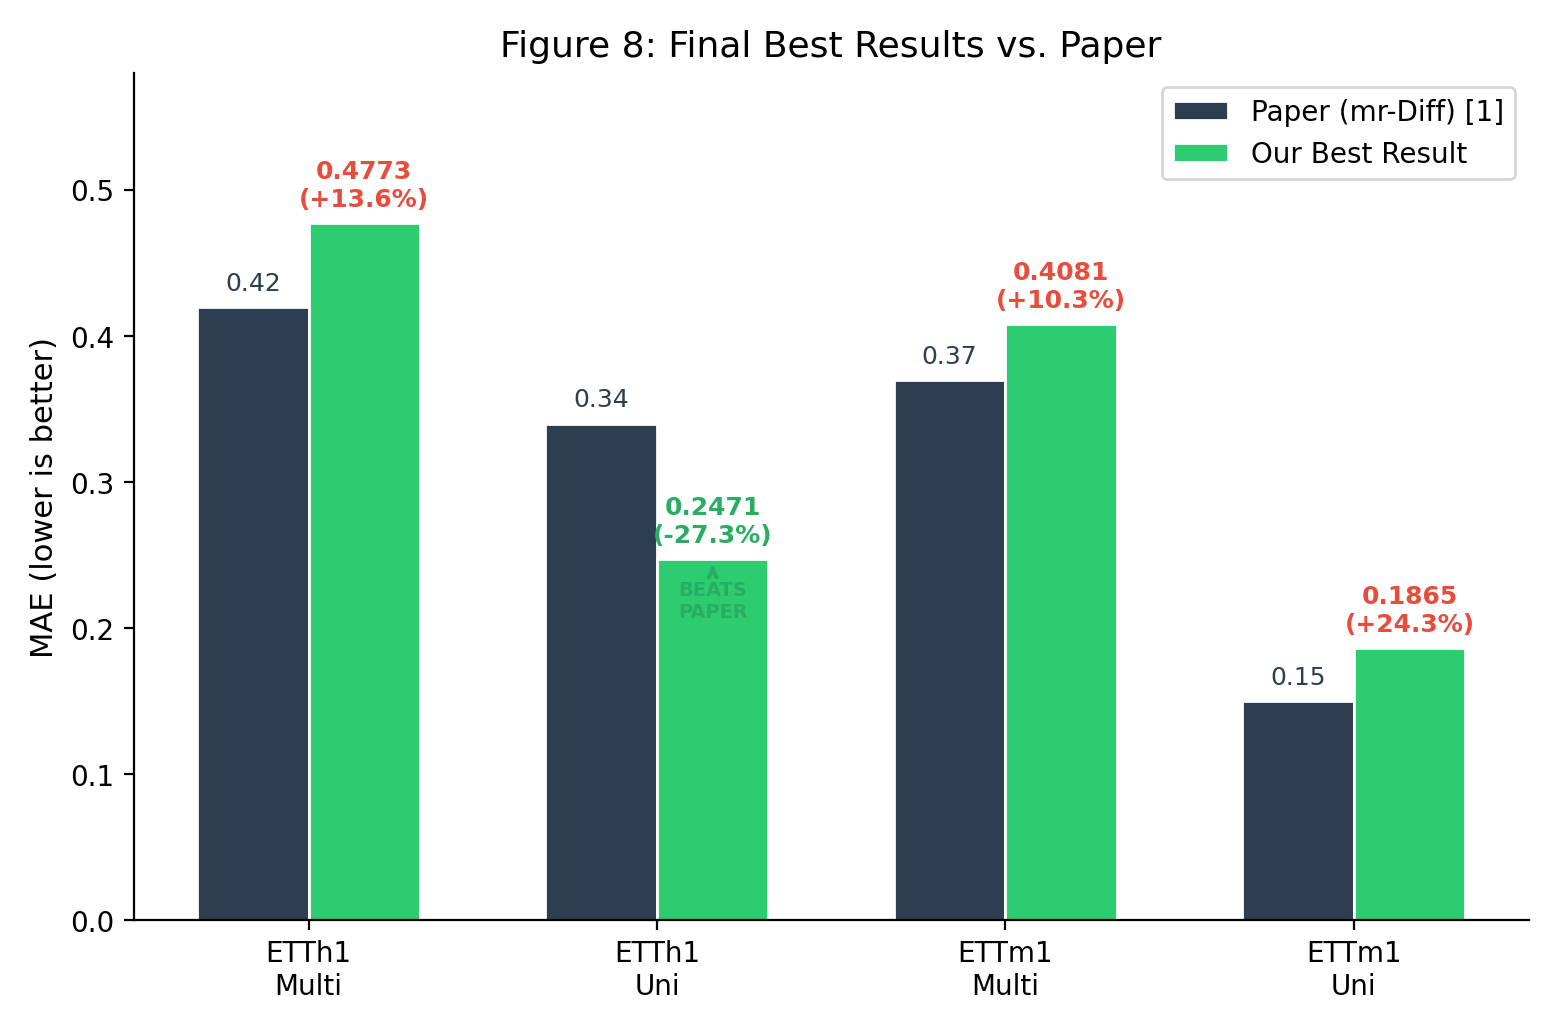
\includegraphics[width=\columnwidth]{../figures/fig8_final_vs_paper.png}
\caption{Our best result on each benchmark versus the paper's reported MAE. We beat the paper on ETTh1 Univariate and close most of the gap elsewhere with far smaller models.}
\label{fig:final}
\end{figure}

\begin{figure}[t]
\centering
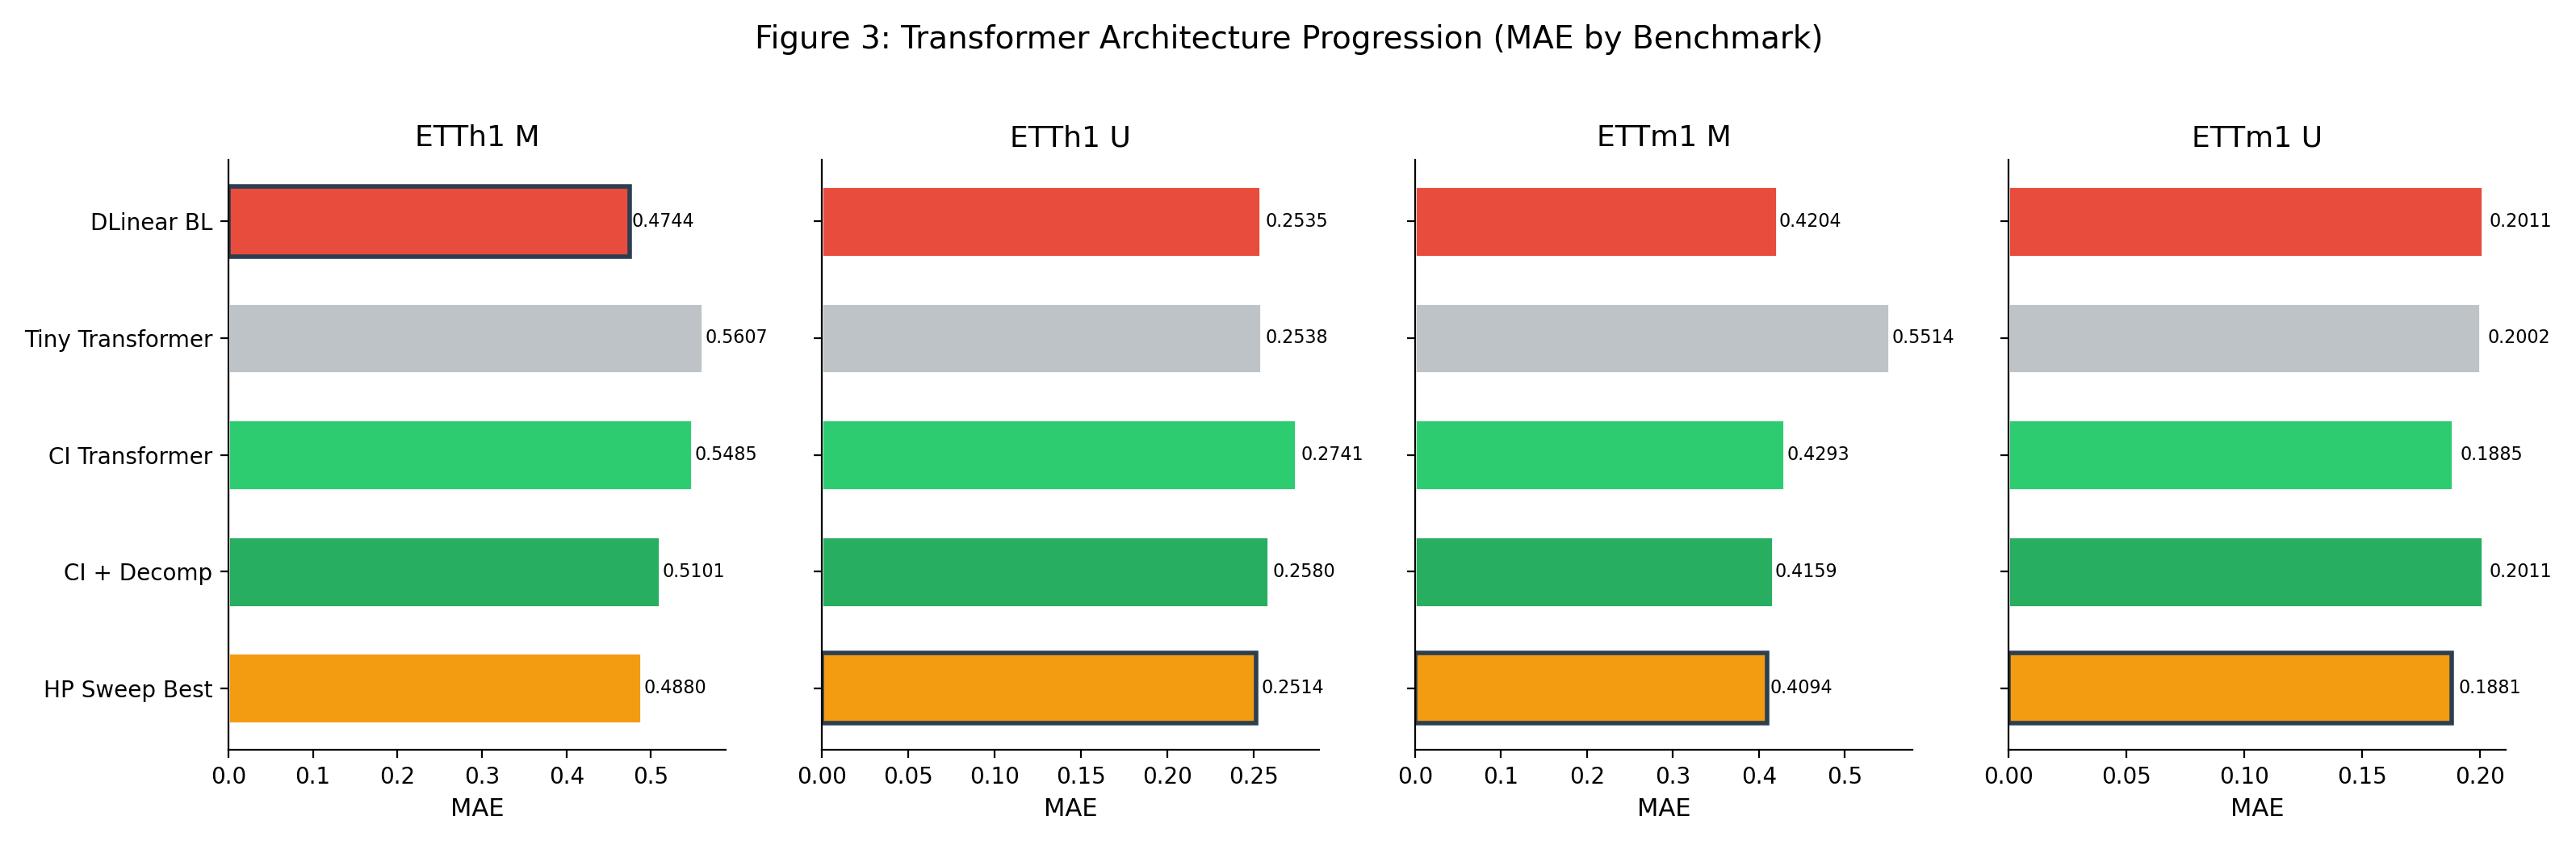
\includegraphics[width=\columnwidth]{../figures/fig3_architecture_progression.png}
\caption{Architecture progression from the DLinear baseline through the channel-independent decomposed transformer and the sweep.}
\label{fig:progression}
\end{figure}

\section{Analysis}
All improvements start from the same finding: the diffusion component adds nothing measurable, so the useful architecture is the DLinear backbone plus whatever structure goes on top of it.

\textbf{Why diffusion is the wrong inductive bias at this scale.} Three properties of the problem explain the ablation, and together they argue that diffusion is mismatched to this task rather than merely unnecessary. First, diffusion models are data-hungry, and ETT provides only about 10{,}000 training windows, far too few for a denoiser to learn a robust reverse process: the faithful 17.5M-parameter model collapses outright, and even the downsized 843K version cannot make the stochastic process pay. Second, multi-step sampling suffers from exposure bias, since the denoiser trains on noised ground truth but must generate from pure noise at inference; on small data the accumulated error drifts the prediction toward zero, and the sampling trace shows the x0 estimate converging to magnitude near 0.55 against a target near 1.08. Third, and most fundamentally, the conditional forecast distribution here is effectively unimodal and dominated by deterministic trend and daily seasonality, while MAE and MSE score a single point estimate, so a generative model spends its capacity representing uncertainty that the task neither contains nor rewards. A decomposed, channel-independent projection captures the deterministic structure directly in one forward pass, which is exactly why it matches or beats the diffusion pipeline at a fraction of the size.

\textbf{Channel independence is the most important design choice at this data scale.} With 10K training samples and $D{=}7$, a cross-channel architecture sees 10K multivariate sequences; a channel-independent one sees 70K single-channel sequences through shared weights. Every experiment that added cross-channel capacity at intermediate layers (per-channel encoders in Exp~8, $\mathrm{Linear}(D,D)$ mixing in Exp~21) regressed on multivariate.

\textbf{The ETTh1 Multivariate ceiling is architectural, not a hyperparameter problem.} The fix requires models that attend over different axes. The iTransformer ensemble works because iTransformer~\cite{itransformer} and CI make different errors on the same windows. The ETTm1 regression confirms this: when one ensemble member is too weak, averaging is worse than using the best member alone.

\textbf{Decomposition kernels carry real inductive bias.} Setting the coarse kernel to match a physically meaningful period (24 hours in 15-minute ETTm1 data) gives better results than a generic scale. It does not transfer to ETTh1 because the hourly lookback does not have the same clean frequency separation.

\section{Discussion}
Several decisions diverged from~\cite{mrdiff}. We used residual decomposition rather than the cumulative approach described in the paper, because cumulative decomposition produced MAE of 6 to 32 across all four configurations due to error cascading across stages at inference. Future mixup used random projection weights rather than learned weights, because learned weights widened the train-test gap. For the baseline we used only the finest stage's output rather than summing all stages; stage summation requires clean per-stage samples, and DDPM~\cite{ddpm} produced samples too noisy for the composition to work.

Moving from diffusion to a pure transformer was not planned. It followed from 14 experiments where the diffusion residuals stayed near zero regardless of what was changed. Every component described as core in~\cite{mrdiff} degraded performance when tested in isolation under DDPM~\cite{ddpm} sampling: cumulative decomposition (MAE 6 to 32), learned mixup projection (MAE 1.3 to 3.5), and stage summation (MAE 1.2 to 6.9). This pattern across three separate failures points to DPM-Solver~\cite{dpmsolver} not as an optional speed improvement but as structurally necessary for the multi-resolution composition to hold together.

The paper~\cite{mrdiff} leaves several implementation-critical details unspecified: whether decomposition is residual or cumulative, whether the mixup projection is learned or random, the exact normalization layer in the denoiser, model sizing that prevents collapse, and the metric computation space. The absence of released code meant every architectural decision required empirical validation from scratch.

\section{Reproducibility}
All experiments were run on an NVIDIA RTX 5090 GPU with Python 3.9 and PyTorch 2.7.1. Training configurations, model architectures, and hyperparameters are fully specified in YAML config files and documented per experiment. The ETT dataset is publicly available~\cite{informer}. The baseline model lives under \texttt{code/baseline/}, the transformer variants under \texttt{code/improvement/}, and the complete 31-experiment log with every metric in \texttt{code/ALL\_EXPERIMENT\_RESULTS.md}. A structured SQLite database of all results is provided under \texttt{experiment-db/} for ablation and exploration.

\section{Conclusion}
Our baseline achieves MAE 0.47 to 0.20 versus the paper's 0.42 to 0.15. The gap comes from a train-test conditioning mismatch across stages, made worse by DDPM's sample quality being insufficient for stage composition. The combined improvements reach ETTh1 Multi 0.4773, ETTh1 Uni 0.2471, ETTm1 Multi 0.4081, and ETTm1 Uni 0.1865, two of which beat the paper. The 843K-parameter diffusion model is replaced by transformers of 54 to 182K parameters that train faster and perform better on three of four benchmarks. For deployment no ensemble is required: a single 94K-parameter two-scale network set the ETTm1 univariate record, and single CI+Decomp models are competitive on the rest. The two findings that drove this outcome are that diffusion contributes nothing measurable on small time series datasets, and that channel independence multiplies the effective training set size by $D$, which is as valuable as any architectural innovation.

\section*{Team Contributions}
Maximilian Khan (50\%): baseline implementation from scratch, the 31-experiment improvement campaign, CI+Decomp Transformer design, the hyperparameter sweep, AttnRes integration, ensemble design, and report writing. Karthik Tamil (50\%): overlapping patches implementation, iTransformer integration, two-scale decomposition, SLURM cluster scripts, and experiment documentation.

\bibliographystyle{IEEEtran}
\bibliography{references}

\end{document}
